\begingroup
\clearpage
\let\clearpage\relax
\vspace*{-16pt}
\chapter[CONCLUSION AND FUTURE WORK]{CONCLUSION AND FUTURE WORK}\label{sec.conclusion}
\endgroup
The contributions of this dissertation are summarized below.

We introduce the maximum mortality rate clique problem, a
novel fractional combinatorial optimization problem defined on a
comorbidity graph derived from EHR data. Given a graph whose vertices
are ICD-coded disease categories and whose edges reflect statistically
significant pairwise co-occurrence measured via the Ochiai
coefficient, MMRCP seeks the $\ell$-frequent clique that maximizes
the mortality rate of the patient population simultaneously diagnosed
with all diseases in the clique. We also introduce a size-restricted
variant and the maximum marginal mortality rate clique problem, which
identifies the diseases whose addition to a known clique most elevates
the mortality rate of the combined cluster. The comorbidity graph used
throughout is constructed from MIMIC-IV using mappings from ICD codes
to disease categories via the CCS and CCSR tools, yielding a graph with
467 vertices and \numprint{8539} edges.

We establish the key theoretical properties of MMRCP. We prove that
the mortality rate function is neither additive nor monotonic, ruling
out simple greedy or local-search strategies and constituting the
fundamental structural obstacle that motivates the solution methods
developed in this dissertation. We establish the computational
hardness of MMRCP through three NP-completeness theorems.

We develop two exact combinatorial algorithms for MMRCP. The first is
a modified Bron--Kerbosch algorithm that enumerates all
$\ell$-frequent cliques while pruning branches that violate the
frequency constraint. The second is a combinatorial branch-and-bound
algorithm that incorporates an upper-bounding scheme to prune
branches whose mortality rate cannot improve upon the current
incumbent, enabling substantially faster search.

We present two MILP formulations for MMRCP. The first linearizes the
fractional mortality rate objective via auxiliary product variables,
and the second applies the Charnes--Cooper transformation. Both are
implemented with delayed constraint generation, but become
intractable as the patient population grows due to the proliferation
of patient-indexed constraints, confirming the need for alternative
strategies on large-scale instances.

To overcome these scalability limitations, we introduce a logic-based
Benders decomposition framework that eliminates all
patient-indexed variables, using only the clique incidence vector and
a scalar representing the mortality rate. Optimality cuts take the
form of simple no-good inequalities anchored at known $\ell$-frequent
cliques, and feasibility cuts are cover inequalities derived from
minimal non-$\ell$-frequent cliques. The reformulation is embedded in
a decomposition branch-and-cut algorithm with a root node relaxation
strengthened by upper-bound-based valid inequalities.

We develop a hybrid LBBD variant that integrates the combinatorial
branch-and-bound algorithm to generate stronger valid inequalities
within the decomposition framework. The combinatorial algorithm is
invoked at branch-and-cut tree nodes on a substantially smaller
induced subgraph, producing cuts that tighten the master problem far
more than the corresponding simple no-good cuts. The hybrid variant
substantially outperforms both the pure LBBD and the direct MILP
formulations across all tested instances, and is the only method to
prove optimality on the largest instances within the time limit.

We further demonstrate the flexibility of the hybrid variant to
incorporate side constraints on the cliques. As an example, we
introduce an age-based constraint that limits the proportion of
patients aged 60 or older across the diseases in the selected clique.
Incorporating this constraint reveals a qualitatively different class
of lethal cliques centered on systemic and metabolic disease
interactions---such as combinations of alcohol-related disorders, liver
disease, and acute renal failure---whose lethality is unlikely to be explained primarily by the elevated baseline mortality of elderly patients. We also introduce a cancer-containing constraint requiring at least one
cancerous diagnosis in the selected clique, yielding clinically
distinct high-mortality clusters; notably, combinations anchored at
secondary malignancies and conditions due to neoplasm treatment are
among the most lethal identified on the complete dataset. Both
constrained variants are solved to optimality across all cohort sizes
and the complete dataset. Side constraints of this form can be
seamlessly incorporated into the hybrid LBBD framework without
modifying the combinatorial branch-and-bound algorithm, underscoring
its advantage.

We apply an adaptation of the modified Bron--Kerbosch algorithm,
extended to enforce a clique-size bound and to enumerate the top-$K$
highest-mortality cliques, to the complete MIMIC-IV dataset of
\numprint{223291} patients, identifying the most lethal disease
cliques across a range of clique sizes. The algorithm scales
efficiently to this population. We further demonstrate the
framework's ability to explore the comorbidity graph broadly by
analyzing a reduced cohort after removing the two most dominant
conditions, revealing a qualitatively different set of high-mortality
comorbidity patterns. The marginal mortality rate analysis, which uses
the same algorithm initialized with a known clique, identifies
diseases whose addition to an existing diagnosis cluster most elevates
mortality risk.

Python implementations of all methods are available in the online repository~\citep{Diss-GithubRepo}.

Parts of this dissertation have appeared in the following publications,
the first published and the second currently under review.
\begin{itemize}
    \item ``Identifying Most Lethal Cliques in Disease Comorbidity
    Graphs,'' \cite{VaghfiMohebbi2025lethalclique}, \textit{IISE
    Transactions on Healthcare Systems Engineering}, 15(2), 183--200.
    Selected by the Editor-in-Chief of \textit{ISE Magazine}.
    \item ``Exact Approaches for the Maximum Mortality Rate Clique
    Problem,'' Preprint available on \hl{Optimization Online}.
\end{itemize}

\paragraph{Limitations.}
We recognize some limitations of this work. The MIMIC-IV dataset is
derived from a single academic medical center, which may limit the
generalizability of the specific disease clusters identified. We note
that while the proposed methods were initially developed and evaluated
on another EHR dataset comprising millions of patient encounters,
access to this dataset was withdrawn during the development of this
work; consequently, those results are not included in the present
study. The one-year post-discharge mortality definition used in
MIMIC-IV means that findings may differ under alternative mortality
windows or definitions, such as in-hospital mortality alone. As with
any study based on coded diagnoses, the quality of results is
sensitive to the completeness and accuracy of ICD coding practices.
External validation using diverse EHR systems and healthcare settings
would strengthen confidence in the robustness of the methods and the
results.

\paragraph{Future Directions.}
The side-constraint framework can be extended to encode other clinically
important requirements based on demographic, socioeconomic, or
treatment-related characteristics, enabling targeted investigations
of specific patient subpopulations. Applying the framework to larger,
multi-institution EHR datasets would support broader validation and
the discovery of previously understudied lethal disease combinations.

In clinical practice, rapid identification of high-mortality disease
combinations can directly inform time-sensitive decisions. A
clinician assessing a patient already carrying several diagnoses may
need to know quickly which additional co-occurring conditions elevate
mortality risk most sharply, in order to prioritize monitoring,
adjust treatment protocols, or initiate early intervention. Exact
methods, while optimal, may be too slow for interactive clinical use.
Developing fast heuristic approaches that can return high-quality
solutions within seconds would make the framework practical for
real-time decision support. Building on this, a natural direction is
the development of a decision-support tool that accepts a
clinician-specified set of diseases and identifies, via a heuristic
engine running in the background, the co-occurring diseases most
associated with elevated mortality in the underlying EHR dataset. A
web-based or locally deployable prototype of such a tool is
illustrated in Figure~\ref{fig.tool}. The development of this tool is an ongoing project by the author.
\begin{figure}[htbp]
    \centering
    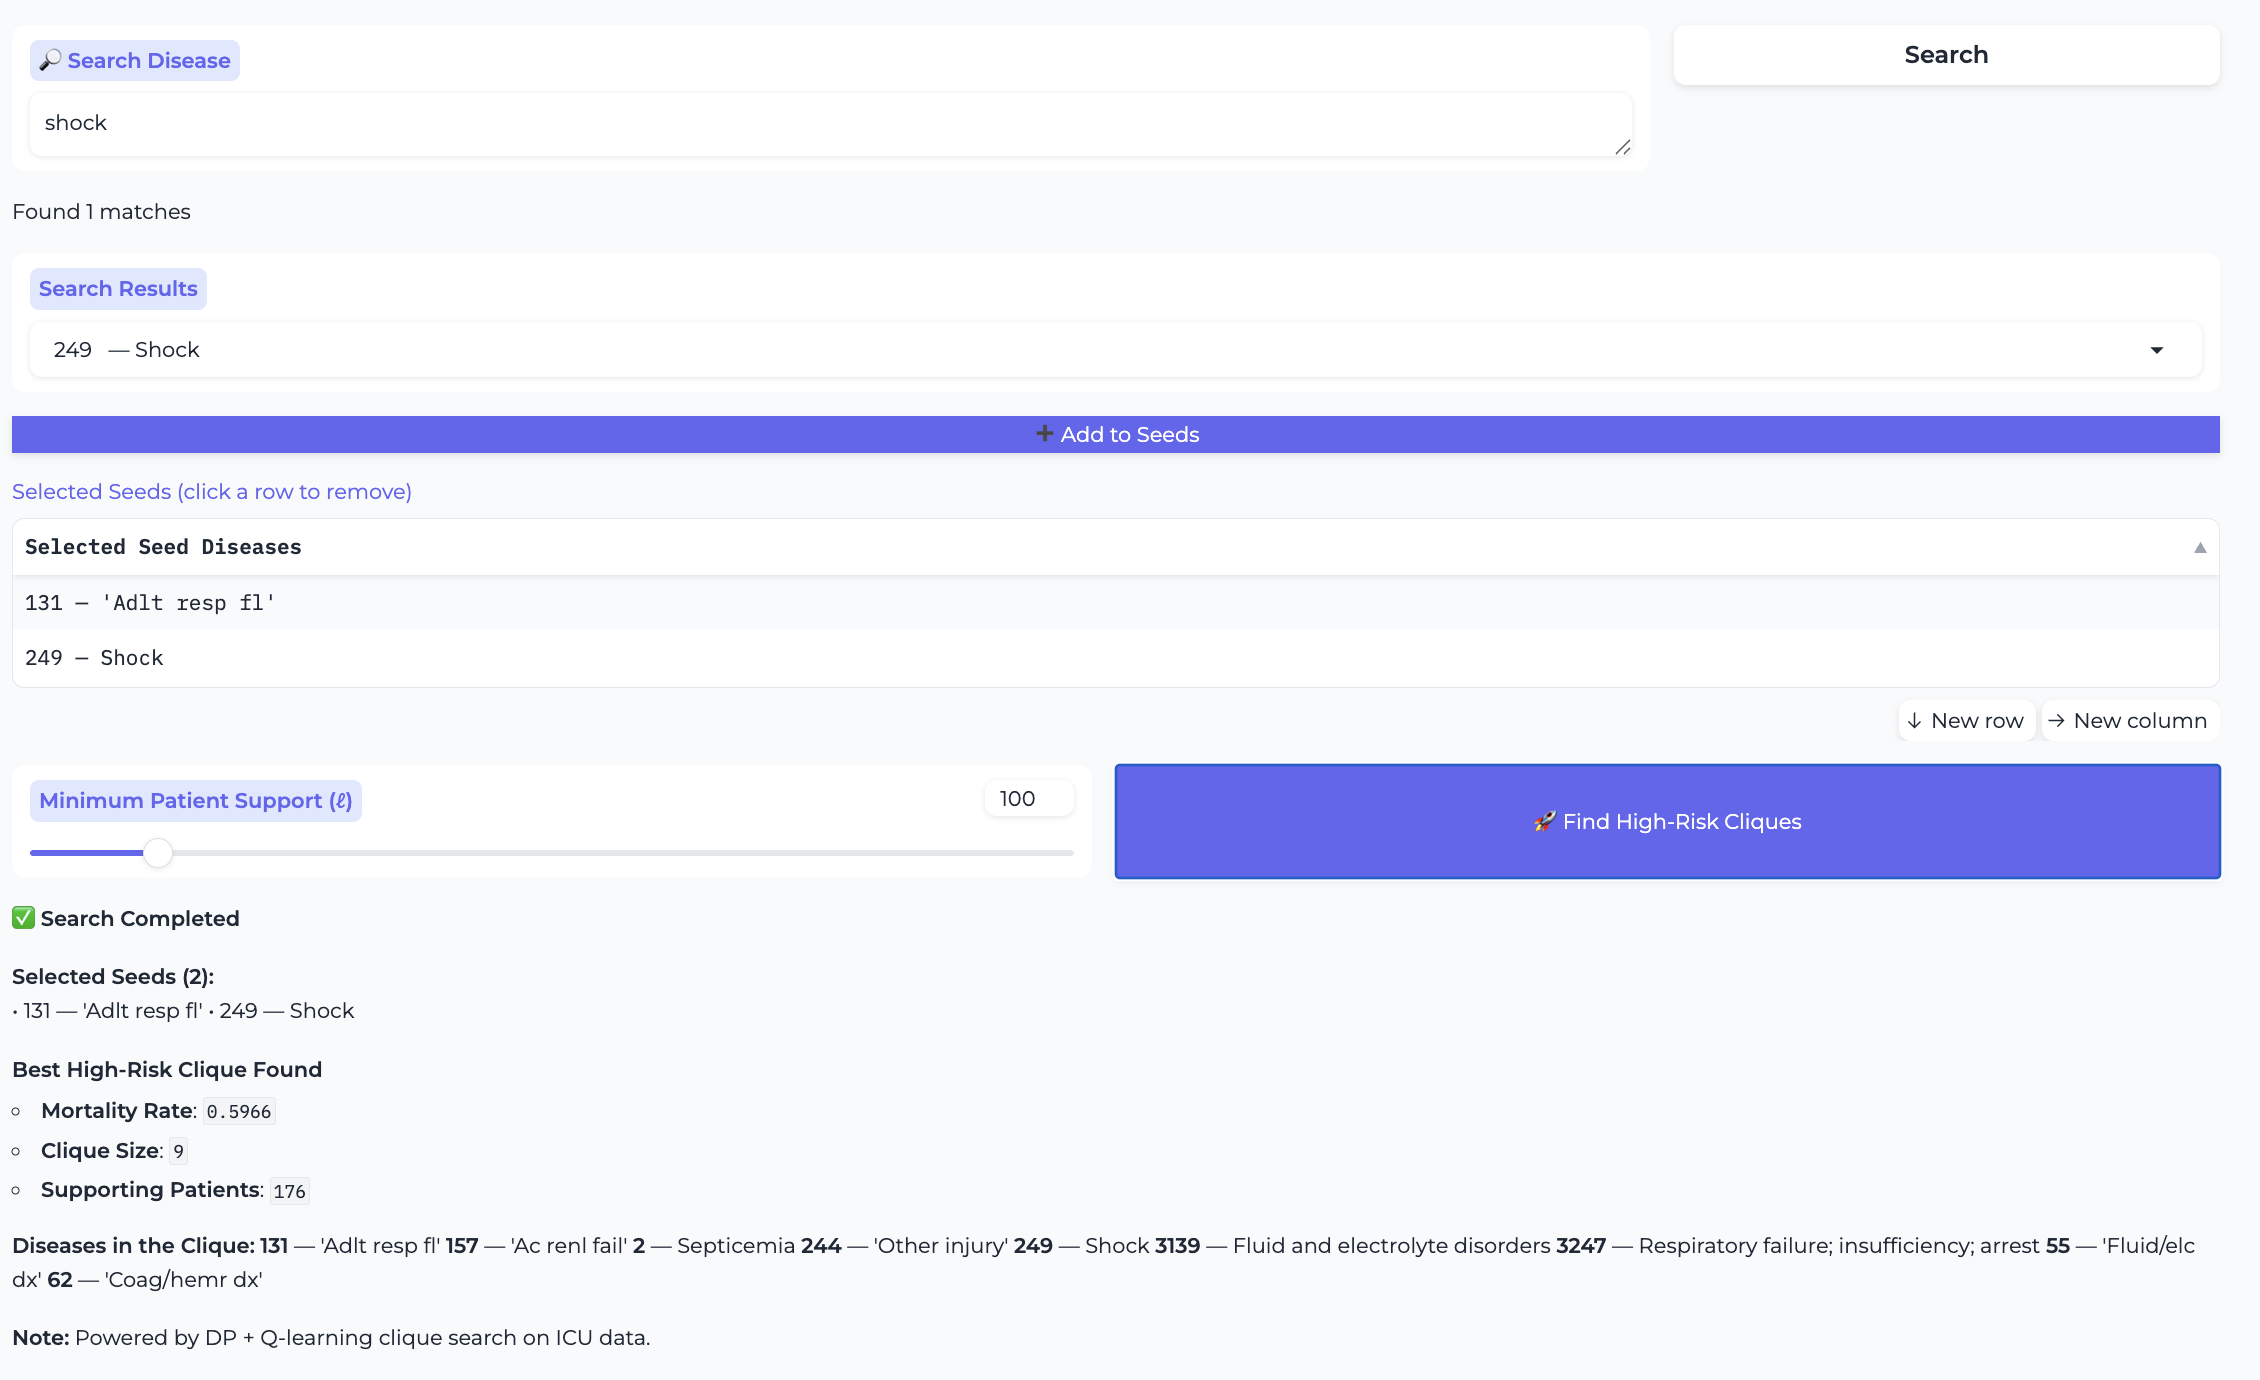
\includegraphics[width=1\textwidth]{Proto.png}
    \caption{Prototype User Interface for Identifying High-Risk
    Disease Cliques}
    \label{fig.tool}
\end{figure}